\documentclass[aps, 12pt]{revtex4}
\usepackage[english]{babel}
\usepackage[utf8]{inputenc}
\usepackage[T1]{fontenc}
% \usepackage{NotesTeX}
\usepackage{subfigure}
\usepackage{tikz}
\usetikzlibrary{arrows}
\usepackage{multirow}
\usepackage{listings}
\usepackage{extarrows}
\usepackage{parskip}
\usepackage{eurosym}
\usepackage{footmisc}
\usepackage{kantlipsum}
\usepackage{algorithm}
\usepackage{algpseudocode}


\def\thesection{\arabic{section}}

\renewcommand{\deg}{^{\circ}}
\newcommand\numberthis{\addtocounter{equation}{1}\tag{\theequation}}
\newcommand{\hksqrt}[2][]{\ \mathpalette\DHLhksqrt{[#1]{#2\,}}}
\def\DHLhksqrt#1#2{\setbox0=\hbox{$#1\sqrt#2$}\dimen0=\ht0
    \advance\dimen0-0.3\ht0
    \setbox2=\hbox{\vrule height\ht0 depth -\dimen0}
    {\box0\lower0.65pt\box2}}

\graphicspath{{figs/}}
\newcommand{\includegraphicsmaybe}[2][]{\IfFileExists{../plots/#2}{\includegraphics[#1]{#2}}{\includegraphics[width=0.7\linewidth]{giffel.jpg}}}



\begin{document}

\author{Håkon Olav Torvik}
\title{\Huge Problem Set 1 \\ \small Math228B Numerical solutions to differential equations}
\affiliation{UC Berkeley}
\date{\today}


\maketitle

\section*{Problem 1a}
The 9-point and 5-point Laplacians are given as

\begin{align*}\label{eq:9ptL}
    \nabla_9^2u_{i,j} = & \frac{1}{6h^2 }[20u_{i,j} -  4u_{i-1,j} -   4u_{i+1,j} -  4u_{i,j-1} - 4u_{i,j+1}
    \\
                        & - 1u_{i+1,j+1} - 1u_{i+1,j-1} - 1u_{i-1,j+1} - 1u_{i-1,j-1}], \numberthis{}
    \\
    \nabla_5^2u_{i,j} = & \frac{1}{h^2}[4u_{i,j} - u_{i-1,j} - u_{i+1,j} - u_{i,j-1} - u_{i,j+1}]
\end{align*}

The dominant error term in the 5-point Laplacian is know, and given by
\begin{equation*}
    \frac{h^2}{12}(u_{xxxx} +u_{yyyy}),
\end{equation*}
with the remaining error goes as $\mathcal{O}(h^4)$.

In the the book, the true solution is applied to the 9-point laplacian before Taylor expanding. This gives the following expression for the 9-point Laplacian
\begin{align*}
    \nabla_9^2u_{i, j} & = \nabla^2 u + \frac{h^2}{12}\left(u_{xxxx} + 2u_{xxyy} + u_{yyyy}\right) + \mathcal{O}(h^4),
    \\
                       & =\nabla^2u +\frac{h^2}{12}(u_{xxxx} + u_{yyyy}) + \frac{h^2}{6}u_{xxyy} + \mathcal{O}(h^4),
    \\
                       & = \nabla_5^2u + \frac{h^2}{6}u_{xxyy} +\mathcal{O}(h^4).
\end{align*}

\section*{Problem 1b}
Solving Laplaces' equation, $\nabla^2u(x,y)=f(x,y)$, using the 9-point Laplacian approximation \eqref{eq:9ptL}, it is re-written
\begin{equation*}
    \nabla_9^2u_{ij} = f_{ij},
\end{equation*}
where
\begin{equation*}
    f_{ij} = f(x_i, y_j) + \frac{h^2}{12} \nabla^2f(x_i, y_j).
\end{equation*}
Using the 5-point Laplacian on $f$ here, the set of equations that needs to be solved are written

\begin{align*}
    [20u_{i,j} - 4u_{i-1,j} - 4u_{i+1,j} - 4u_{i,j-1} - 4u_{i,j+1} - 1u_{i+1,j+1} - 1u_{i+1,j-1} - 1u_{i-1,j+1} - 1u_{i-1,j-1}] & =
    \\
    6h^2\left(f_{ij} -\frac{1}{12}[4f_{i,j} - f_{i-1,j} - f_{i+1,j} - f_{i,j-1} - f_{i,j+1}] \right)                            & .
\end{align*}

The function \texttt{assemblePossion} from the course page is modified to implement this, in fuction \texttt{Poisson9(n, f, g)} on line 54 in my code submission file. \texttt{assemblePossion} is also a possible to call with same signature, in case the name was important. To test that I get 4th order convergence, I use the test-function from the course page with known exact solution and finds the maximum relative error for different grid sizes. I plot the log of the errors against the log of the step-length $h$, such that the slope $\lambda$ is the convergence rate $\mathcal{O}(h^{\lambda})$. This is done for both the 9-point stencil, as well as the 5-point stencil. As can be seen in Figure \ref{fig:gridRef}, the 9-point stencil is indeed 4th order accurate, while the 5-point is 2nd order.

\begin{figure}
    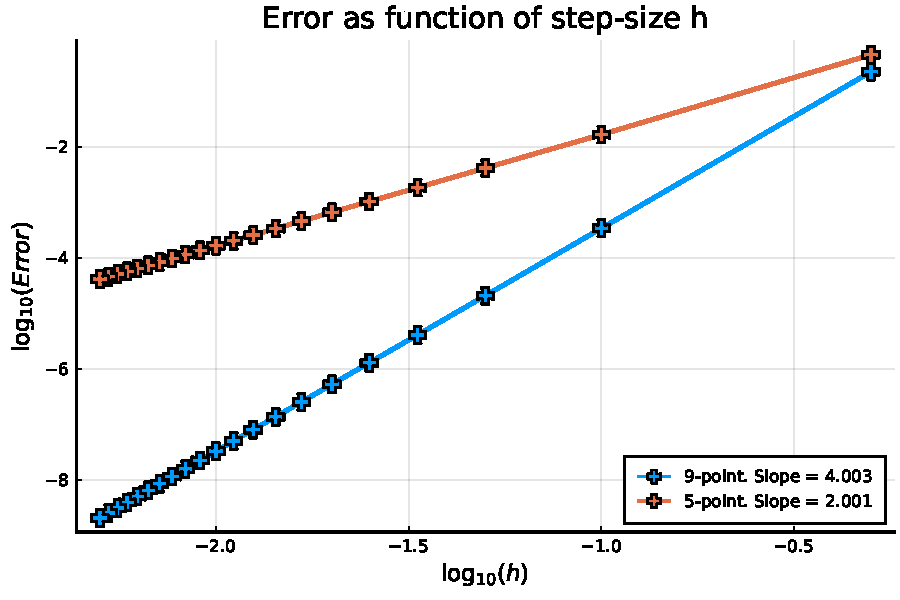
\includegraphics[width=0.8\linewidth]{gridRefinement.pdf}
    \caption{Log-log plot of relative error against step-length for 5-point and 9-point Laplacian stencil, to show the convergence rates of both. The 5-point goes as $\mathcal{O}(h^2)$, while the 9-point as $\mathcal{O}(h^4)$, which is as expected. The 2 points with highest step-length are excluded from the estimation of the slope, in order to avoid inaccuracies for large $h$.}
    \label{fig:gridRef}
\end{figure}


\section*{problem 2a}
The mapping
\begin{align*}
    T = \begin{cases}
        \xi(x, y) = \frac{x}{B/2 + Ay/H} = \frac{x}{\gamma'}, \hspace{4mm} \gamma'(x, y) \equiv B/2 + Ay/H,
        \\
        \eta(x, y) = y / H,
    \end{cases}
\end{align*}
is one transform from $\Omega$ to the unit square $\hat{\Omega}$. The the inverse transform is
\begin{align*}
    T^{-1} = \begin{cases}
        x(\xi, \eta) = \xi\gamma, \hspace{4mm}\gamma(\xi, \eta) \equiv B/2 + A\eta,
        \\
        y(\xi, \eta) = H\eta.
    \end{cases}
\end{align*}

\newcommand{\xegamma}{\gamma(\xi, \eta)}

In $\Omega$, Poissons equation to solve looks like
\begin{equation*}
    -(u_{xx} + u_{yy}) = 1,
\end{equation*}

while in $\hat{\Omega}$, it takes the shape
\begin{equation}\label{eq:ddu}
    au_{\xi\xi}-2bu_{\xi\eta}+cu_{\eta\eta} + du_{\eta}+eu_{xi} = -J^2f,
\end{equation}
where $a, b, c, d, e, J$ are functions of the first and second derivatives of $x$ and $y$ w.r.t. $\xi$ and $\eta$. These derivatives that do not evaluate to 0 are as follows:
\begin{align*}
    x_{\xi} = \gamma \hspace{3mm} x_{\eta} = A\xi \hspace{3mm} y_{\eta} = H \hspace{3mm} x_{\eta\xi} = A
\end{align*}

Using the definitions in the lecture slides, I find that the expressions for the functions of $\xi$ and $\eta$ are given by
\begin{align*}
    \alpha  = -2bA  \hspace{5mm} & \hspace{5mm} \beta   = 0
    \\
    a    = A^2\xi^2 + H^2 \hspace{5mm} & \hspace{5mm} b  = A\xi\gamma
    \\
    c   = \gamma^2\hspace{5mm} & \hspace{5mm} e    = 2A^2\xi
    \\
    d     = 0 \hspace{5mm} & \hspace{5mm}J   = H\gamma
\end{align*}

The Dirichlet boundary conditions stay the same in the computational domain, that is
\begin{equation*}
    u = 0 \hspace{2mm} \text{for $P'_1P'_2$ and $P'_2P'_3$}.
\end{equation*}

The von Neumann condition at $P'_1P'_4, \xi=0$, is given with the normal derivative, and the normal vector is unchanged. Thus
\begin{align*}
    \frac{du}{dn} = \frac{du}{d\xi} = 0
\end{align*}
where I have used a 3-point boundary stencil to approximate the derivative.

At $P'_3P'_4, \eta=1$, the normal derivative is given by
\begin{equation*}
    \frac{\partial u}{\partial n} = \frac{1}{J} \left[(y_{\eta}n^x-x_{\eta}n^y)u_{\xi}+(-y_{\xi}n^x+x_{\xi}n^y)u_{\eta}\right]
\end{equation*}
where
\begin{equation*}
    (n^x, n^y)= \frac{1}{\hksqrt{x_{\xi}^2+y_{\xi}^2}}(-y_{\xi}, x_{\xi}) = (0, 1),
\end{equation*}
such that
\begin{equation*}
    \frac{\partial u}{\partial n} = \frac{1}{J}\left[-A\xi u_{\xi}+\gamma u_{\eta}\right] =\frac{-A\xi}{J}u_{\xi}+\frac{1}{H}u_{\eta}.
\end{equation*}

\section*{Problem 2b}
With all the expressions in the previous secion, I now have all that is needed to discretize the computational domain and write down the systems of equations to solve the system.

First, using $\Delta\xi=\Delta\eta=h=1/n$, we have $\xi\rightarrow\xi_i=ih, \eta\rightarrow\eta_j=jh$ for $i,j\in[0, n]$. Then, a function $g(\xi, \eta)\rightarrow g(\xi_i, \eta_j) = g(i, j) = g_{i,j}$. Setting $f_{ij} =1$, and using 2nd order approximations for the derivatives in \eqref{eq:ddu}, the equations for the interiour points are written

\begin{align*}
    -J_{i,j}^2h^2 = & \big[a_{ij}(u_{i-1, j}-2u_{i,j}+u_{i+1,j}) -\frac{b_{i,j}}{2}(u_{i-1,j+1}+u_{i+1,j-1}-u_{i-1,j-1}-u_{i+1,j+1})
    \\
                    & + c_{ij}(u_{i, j-1}-2u_{i,j}+u_{i,j+1}) + \frac{d_{i,j}}{2}(u_{i,j+1}-u_{i,j-1})+ \frac{e_{i,j}}{2}(u_{i+1,j}-u_{i-1,j})\big]
\end{align*}

For the boundaries, we have
\begin{align*}
    j=0 \lor i=n \Rightarrow & u_{i, j} = 0                                                                     &  & \text{Derichlet at} P'_1P'_2\land P'_2P'_3.
    \\
    i = 0 \Rightarrow        & u_{\xi} \approx \frac{1}{h^2}\left[-1.5u_{i,j}+2u_{i+1,j}-0.5u_{i+2,j}\right]=0, &  & \text{von Neumann at} P'_1P'_4.
    \\
    j =n\Rightarrow          & \frac{-A\xi_i}{J_{i,j}}\frac{1}{2h^2}\left[u_{i+1,j}-u_{i-1j}\right] +
    \\
                             & \frac{1}{H}\frac{1}{h^2}\left[-1.5u_{i,j}+2u_{i,j-1}-0.5u_{i,j-2}\right]=0       &  & \text{von Neumann at} P'_3P'_4.
\end{align*}
3 of the corners are handled by the first case and set to $0$, while the last is handled by the second case, using a left boundary stencil.

These equations can be written simply as $Au=b$. When we have the solution $u$, the flowrate $\hat{Q}$ in the computational domain, which is an intergral over the domain, can be approximated by the 2D-trapezoidal rule, a 2nd order method, as such: \cite{trap}
\begin{align*}
    \hat{Q} = & \iint_{\hat{\Omega}}u_{i,j}d\xi d\eta
    \\
    =         & \frac{h^2}{4}\left[u_{0,0}+u_{0,n}+u_{n,0}+u_{n,n} + 2\left(\sum_iu_{i,0}+\sum_iu_{i,n}+\sum_ju_{0,j}+\sum_ju_{n,j}\right)+4\sum_{i,j}u_{i,j} \right]
\end{align*}

\section*{Problem 2c}

The function \texttt{buildA(L, B, H, n)} in my code constructs the matrix A, vector b as well as the matricies for the physical grid $x$ and $y$. \texttt{channelflow(L, B, H, n)} solves $Au=b$, and plots the result. For $H=1, L=3, B=0.5, n=20$, the resulting contour and grid is shown in Figure \ref{fig:contour}. The figure shares a great resembelance with the figure in the problem set, so I am confident my implementation is at least mostly correct.

\begin{figure}
    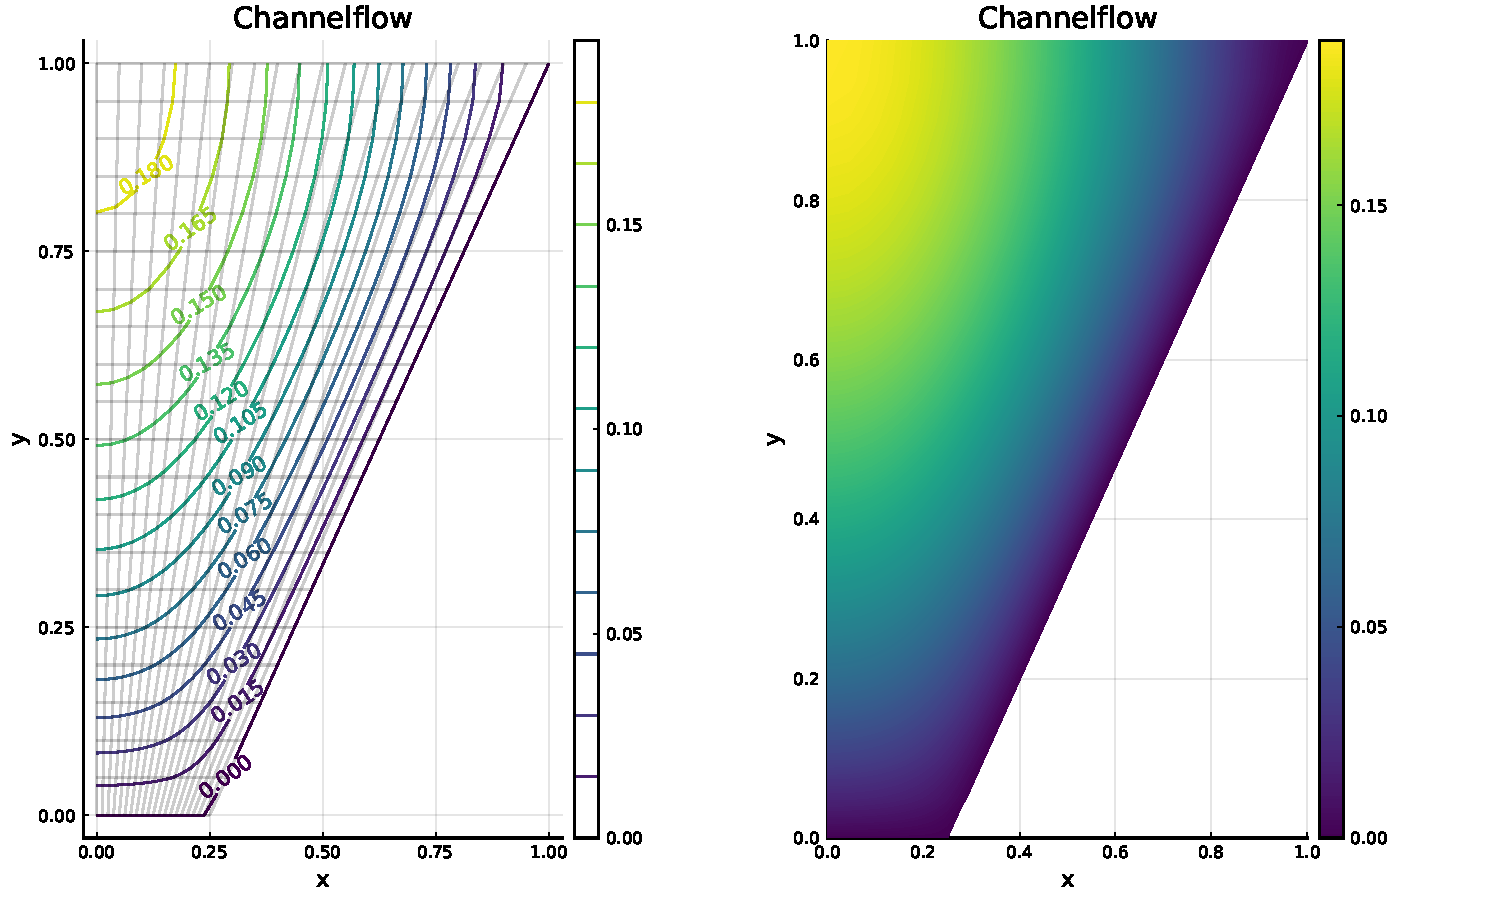
\includegraphics[width=\linewidth]{contour.pdf}
    \caption{Left: unfilled contour with grid of flow in channel. Right: Filled contour of the same simulation.}
    \label{fig:contour}
\end{figure}

\section*{Problem 2d}
For different values of $B$, I calculate the flowrate $\hat{Q}$ for increasing number of points in the discretization, to estimate the convergence rate. As I dont have the exact solution, I let $Q_{true}\equiv Q(n=640)$, and calcuate the relative error for $n=10*2^k, k\in[1:6]$. I plot the results in a log-log plot as in Problem 1b. This is shown in Figure \ref{fig:converge}, for $B=0,0.5,1$ in separate plots. We see that in all cases, the convergence is somewhat better than 2nd order. There is no big difference for the different values of $B$, neither for the slope nor the value of the error.

The flowrate is similar for the case of $B=0$ and $B=1$, and highest for $B=0.5$. This makes sense physically, as this corrosponds to the shape of the chanel with the largest cross-sectional area (among those 3 values. $B=L-H\hksqrt{16/3}\approx0.69$ is the global maximum.)


\begin{figure}
    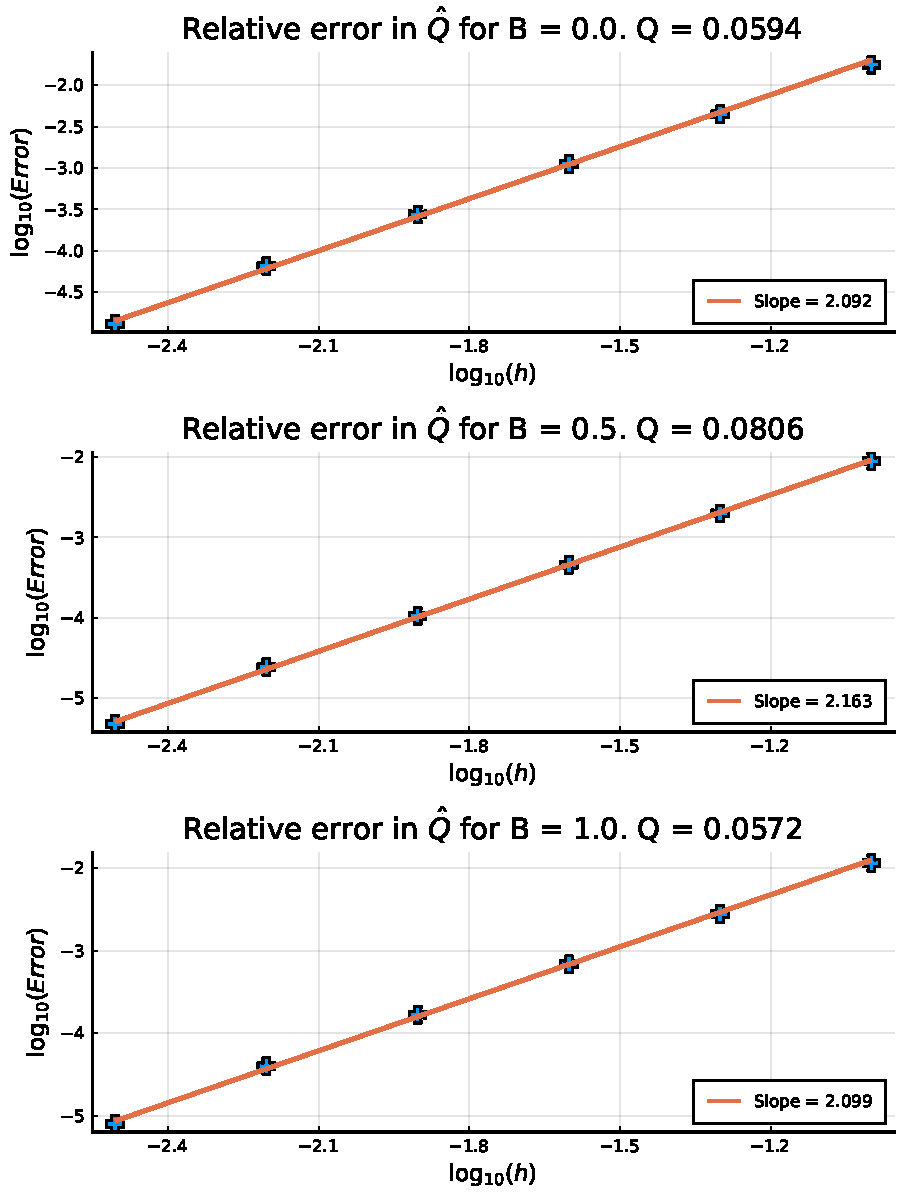
\includegraphics[width=\linewidth]{convergence.pdf}
    \caption{Convergence of error in $\hat{Q}$ for different values of $B$. The first point is excluded in the estimation of the slope to aviod large inaccuracies when $h$ is big.}
    \label{fig:converge}
\end{figure}


\section*{Problem 3}
The PDE
\begin{equation*}
    u_t =\kappa u_{xx} - \gamma u
\end{equation*}
can be solved with the $\theta$-parameterized scheme
\begin{equation*}
    U_j^{n+1} = U_j^n + \frac{k\kappa}{2h^2}\left[U_{j-1}^n - 2U_j^n + U_{j+1}^n + U_{j-1}^{n+1} -2U_j^{n+1}+U_{j+1}^{n+1} \right] - k\gamma \left[(1-\theta)U_j^n+\theta U_j^{n+1}\right].
\end{equation*}

Setting $\gamma = 0$ gives the heat equation which we know has a local truncation error of $\mathcal{O}(h^2)$, so to study the local truncation error in this PDE, I ignore that part by setting $\kappa =0$.
We then get
\begin{align*}\label{eq:p3}
    U_j^{n+1}=                 & U_j^n - k\gamma\left[(1-\theta)U_j^n+\theta U_j^{n+1}\right]
    \\
    (1+k\gamma\theta)U_j^{n+1} & = [1-k\gamma(1-\theta)]U_j^n.
    \\
    (1+k\gamma\theta)U(x, t+k) & = [1-k\gamma(1-\theta)]U(x,t).\numberthis{}
\end{align*}

Taylor expanding the left side as
\begin{align*}
    U(x, t+k) \approx  U+kU_t+\frac{k^2}{2}U_{tt}+\mathcal{O}(k^3).
\end{align*}

From the original PDE, we know
\begin{align*}
    u_t    & =-\gamma u
    \\
    u_{tt} & =(u_t)_t = (-\gamma u)_t= -\gamma u_t = \gamma^2u
\end{align*}

Inserting this into \eqref{eq:p3}, and subtracting the two sides from eachother gives the local truncation error
\begin{align*}
    \tau & = (1+k\gamma\theta)\left(U-k\gamma U+\frac{k^2\gamma^2}{2}U+\mathcal{O}(k^3)\right) - [1-k\gamma(1-\theta)]U
    \\
         & = (1+k\gamma\theta)\left(-k\gamma U+\frac{k^2\gamma^2}{2}U+\mathcal{O}(k^3)\right) + k\gamma U
    \\
         & = k^2\gamma^2\theta U + \frac{k^2\gamma^2}{2}U +\mathcal{O}(k^3)
    \\
         & \begin{cases}
        \mathcal{O}(k^3), \hspace{3mm} \theta = \frac{1}{2}
        \\ \mathcal{O}(k^2), \hspace{3mm} \text{otherwise}
    \end{cases}
\end{align*}

The global error is 1 order lower, and bringing back in the error for $\kappa\neq0$, we get that the method is $\mathcal{O}(k^p+h^2)$ accurate, where $p=2$ for $\theta=\frac{1}{2}$ and $p=1$ otherwise.






\begin{thebibliography}{99}
    \bibitem{trap} Math StackExchange, \textit{Derivation of 2D Trapezoid Rule}, retrieved at the internet from \textit{https://math.stackexchange.com/questions/2891298/derivation-of-2d-trapezoid-rule} at 02/02/2022
\end{thebibliography}

\end{document}

